\documentclass{IEEEtran}

\usepackage{mathtools}
\usepackage{graphicx}
\usepackage{subfig}
\usepackage{verbatim}
\usepackage{algpseudocode}
\usepackage{natbib}
\usepackage{url}
\usepackage{listings}
\usepackage[spanish]{babel}
\usepackage[utf8x]{inputenc}
\usepackage{float}
\usepackage{array}
\usepackage{booktabs}
%\setcounter{MaxMatrixCols}{16}

\begin{document}

\title{Informe Tarea No 3}
\date {Mayo de 2013}
\author{\IEEEauthorblockN{Tatiana Lopez Guevara \\}
\IEEEauthorblockA{Universidad Tecnológica de Pereira\\
tatiana@sirius.utp.edu.co }}
\maketitle


\begin{abstract}
El presente documento explica los resultados obtenidos en la implementación del algoritmo
para extracción de puntos de interés o POI (Points of Interest) basado en el método de Harris.
\end{abstract}

\begin{IEEEkeywords}
Computer Vision
\end{IEEEkeywords}

\section{Introducción}

A continuación se mostrará el resultado obtenido en cada paso del algoritmo
sobre el primer par de imágenes de prueba (figura \ref{fig:img1}) y el análisis 
correspondiente en cada caso. Como se puede observar, la diferencia entre la izquierda
y la derecha de la figura consiste en una simple rotación y un leve cambio en el brillo.
En la última sección se mostrará el resultado
obtenido sobre otros pares de imágenes con diferentes distorciones
y los valores de los parámetros empleados
en cada caso.


\begin{figure}[H]
\caption{Imágenes iniciales}
\centering

\includegraphics[width=8.9cm,natwidth=1200,natheight=450]{figs/img1.png}
\label{fig:img1}
\end{figure} 

\section{Suavizado Gausiano}
Para el cálculo del tamaño kernel Gausiano la referencia de corte se tomó en
$3 \sigma$. Por lo tanto, el tamaño total está dado por el pixel central 
más 2 veces la referencia de corte aproximada al entero próximo más grande (\ref{eq:wgaus}).

\begin{equation}
WG_{N} = 1 + 2 * ceil( 3 * \sigma )
\label{eq:wgaus}
\end{equation} 

En la versión discretizada de la función Gausiana (\ref{eq:gaus}) , el valor de A se toma de tal forma
que los valores de los extremos del kernel -los más alejados de la media- no queden
con un valor muy despreciable. En este caso se tomó un valor de 300.

\begin{equation}
\begin{aligned}
G(x,y) = A e^{\frac{-(x^2 + y^2)}{2 \sigma^2}}
\label{eq:gaus}
\end{aligned}
\end{equation} 

A continuación se muestran los kernels (tablas \ref{tb:gaus1}, \ref{tb:gaus06}) 
generados para una desviación de $0.6$ y $1.0$ respectivamente.

\begin{table}[H]
\centering
\begin{tabular}{|*7c|}
\hline
 0.037& 0.451& 2.021& 3.333& 2.021& 0.451& 0.037\\
 0.451& 5.495& 24.625& 40.601& 24.625& 5.495& 0.451\\
 2.021& 24.625& 110.364& 181.959& 110.364& 24.625& 2.021\\
 3.333& 40.601& 181.959& 300.000& 181.959& 40.601& 3.333\\
 2.021& 24.625& 110.364& 181.959& 110.364& 24.625& 2.021\\
 0.451& 5.495& 24.625& 40.601& 24.625& 5.495& 0.451\\
 0.037& 0.451& 2.021& 3.333& 2.021& 0.451& 0.037\\
\hline
\end{tabular}
\caption{Kernel Gausiano $\sigma = 1.0$ - $WG_{N}=7$}
\label{tb:gaus1}
\end{table} 

Sobre la imágen de la prueba 1 se aplicó un kernel con $\sigma=0.6$ 
obteniendo el resultado de la figura \ref{fig:gaus06}.

\begin{figure}[H]
\caption{Filtro Gausiano $\sigma = 0.6$}
\centering
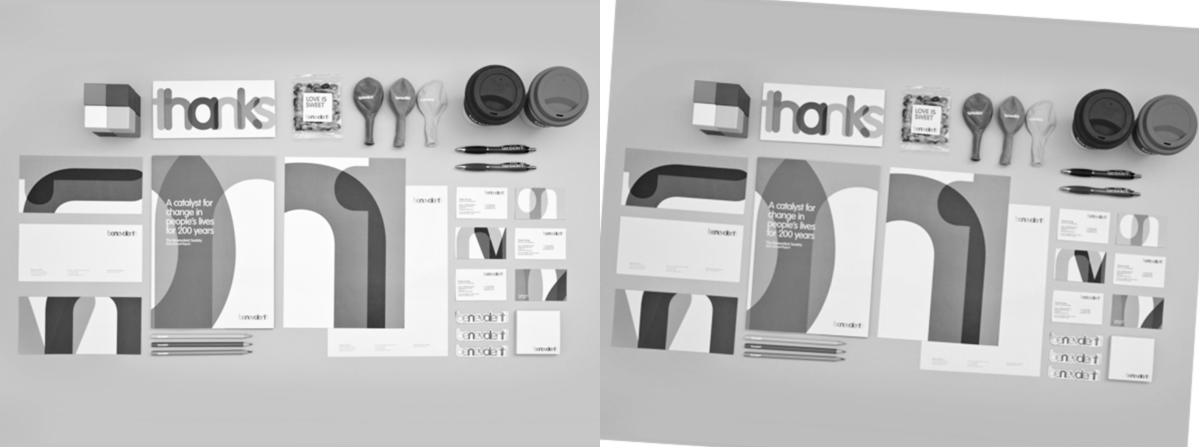
\includegraphics[width=8.9cm,natwidth=1200,natheight=450]{figs/gaus06.png}
\label{fig:gaus06}
\end{figure} 

\begin{table}[H]
\centering
\begin{tabular}{|*5c|}
\hline
 0.004& 0.289& 1.160& 0.289& 0.004\\
 0.289& 18.653& 74.806& 18.653& 0.289\\
 1.160& 74.806& 300.000& 74.806& 1.160\\
 0.289& 18.653& 74.806& 18.653& 0.289\\
 0.004& 0.289& 1.160& 0.289& 0.004\\
\hline
\end{tabular}
\caption{Kernel Gausiano $\sigma = 0.6$ - $WG_{N}=5$}
\label{tb:gaus06}
\end{table}

Finalmente, una vez aplicado el kernel gausiano sobre la imágen, se procedió a 
normalizar la escala de colores obtenida para dejarla en un rango de 0 (negro) 
a 1 (blanco)
mediante (\ref{eq:norm}) \cite{nixon2008feature}.

\begin{equation}
P(x,y) = \frac{P(x,y) - P_{min}}{P_{max} - P_{min}}
\label{eq:norm}
\end{equation} 

\section{Detector de Bordes de Sobel}
El operador de sobel combina un suavizado gausiano u óptimo 
en un eje con una diferenciación en el otro eje \cite{nixon2008feature}.
Esto se realiza mediante la convolución de la imágen con los siguientes
kernels:

\begin{table}[H]
\centering
\begin{tabular}{|*3c|}
\hline
-1 & 0 & 1 \\
-2 & 0 & 2 \\
-1 & 0 & 1 \\
\hline
\end{tabular}
\caption{Kernel de Sobel Sh}
\label{tb:sh}
\end{table}

\begin{table}[H]
\centering
\begin{tabular}{|*3c|}
\hline
1 & 2 & 1 \\
0 & 0 & 0 \\
-1 & -2 & -1 \\
\hline
\end{tabular}
\caption{Kernel de Sobel Sv}
\label{tb:sv}
\end{table}

Al aplicarlo sobre la imágen, se obtiene la figura \ref{fig:sobel}.

\begin{figure}[H]
\caption{Detector de bordes de Sobel}
\centering
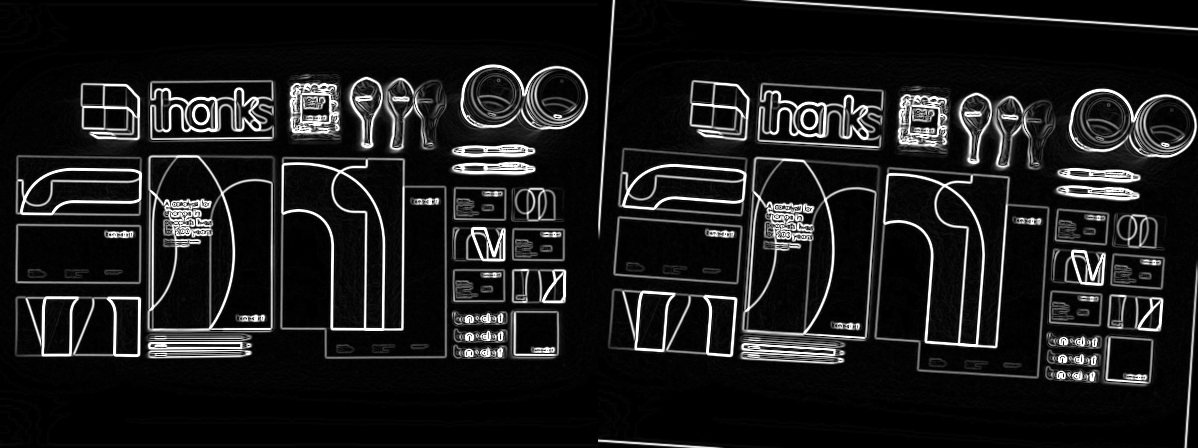
\includegraphics[width=8.9cm,natwidth=1200,natheight=450]{figs/sobel.png}
\label{fig:sobel}
\end{figure} 


\section{Detector de Esquinas de Harris}
Como se puede apreciar en (\ref{eq:rmat}) y en la figura \ref{fig:rmat}, el 
detector de esquinas de Harris penaliza más a los bordes que a las 
regiones planas y realza las esquinas.

\begin{equation*}
\begin{aligned}
C =\begin{bmatrix} \displaystyle\sum_W dx^2 & \displaystyle\sum_W dx dy \\
				   \displaystyle\sum_W dx dy & \displaystyle\sum_W dy^2 \end{bmatrix}
\end{aligned}
\end{equation*} 

\begin{equation}
R = det(C) - k*trace(C)^2
\label{eq:rmat}
\end{equation} 

\begin{figure}[H]
\caption{Interpretación de valores de R. Fuente \cite{cornerdetection}}
\centering
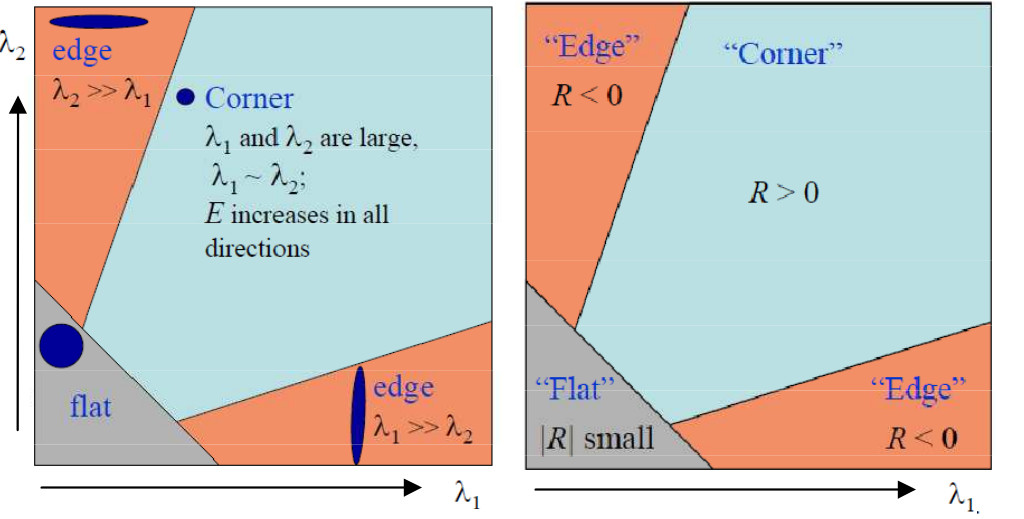
\includegraphics[width=7.1cm,natwidth=1024,natheight=519]{figs/rmat.jpg}
\label{fig:rmat}
\end{figure}

Esto se ve reflejado en la imágen después de normalizar la escala
de colores, donde los bordes se ven negros (valores mínimos),
las regiones planas se ven grises y las esquinas se ven blancas (valores máximos).

\begin{figure}[H]
\caption{Detector de esquinas de Harris}
\centering
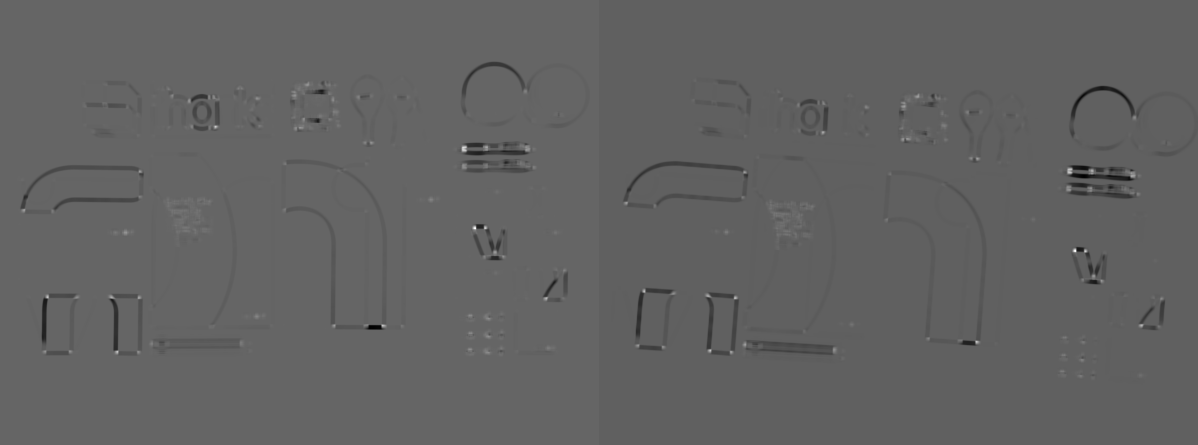
\includegraphics[width=8.9cm,natwidth=1200,natheight=450]{figs/harris.png}
\label{fig:harris}
\end{figure}

\subsection{Pruebas de Umbrales}

El umbral seleccionado para el valor $k$ de la ecuación (\ref{eq:rmat}) 
fue el de 0,09, ya que con éste se detectaban la mayor cantidad de esquinas significativas
en la imágen. Un valor más grande, detectaba mucha redundancia y empezaba a 
marcar como esquinas cosas que no lo eran y volvía el proceso de hallar correspondencias
demasiado lento (\ref{tb:kharris}) .

\begin{table}[H]
\centering
\begin{tabular}{*3c}
\toprule
Valor Umbral & Pts Img1 & Pts Img2\\
\midrule
0,06 & 380 & 324\\
0,07 & 618 & 520\\
0,08 & 1297 & 1051\\
0,09 & 6514 & 4536\\
0,1 & 261760 & 261064 \\
\bottomrule
\end{tabular}
\caption{Valores para $k$  Harris.}
\label{tb:kharris}
\end{table} 

Ahora, teniendo este valor de $k$ fijo, se varió el 
valor de umbral contra el que se compara el valor de $R$
(\ref{tb:rharris}) .
El valor seleccionado fue el de $R>0.4$ por los
mismos factores explicados para el valor de $k$.

\begin{table}[H]
\centering
\begin{tabular}{*3c}
\toprule
Valor Umbral & Pts Img1 & Pts Img2\\
\midrule
0,60 & 15 & 12\\
0,50 & 46 & 44\\
0,40 & 181 & 155\\
0,35 & 135195 & 111758\\
\bottomrule
\end{tabular}
\caption{Valores de Umbral para R.}
\label{tb:rharris}
\end{table} 

\section{Correspondencias Putativas}
\subsection{Sum of Squared Differences - SSD}

El valor del SSD sobre una ventana es 0 si ambas
muestras son iguales y grande entre más diferentes sean. 
Por lo tanto, entre menor sea
el valor, más similares serán las imágenes. 
Para establecer el valor del umbral sobre el que se iba 
a trabajar, se tomaron diferentes muestras (tabla \ref{tb:tssd})
y se ve que los 3 primeros valores medidos no alcanzan
a tomar suficientes correspondencias. Así mismo, en los 2 
últimos valores no hay un aumento significativo y por lo tanto
el valor seleccionado fue 0,04.

\begin{table}[H]
\centering
\begin{tabular}{*3c}
\toprule
Valor Umbral & Corresp. Detectadas\\
\midrule
0,10 & 2\\
0,20 & 16\\
0,30 & 58\\
0,40 & 85\\
0,50 & 97\\
0,60 & 111\\
\bottomrule
\end{tabular}
\caption{Valores de Umbral para SSD.}
\label{tb:tssd}
\end{table} 

El resultado es el mostrado en la figura \ref{fig:ssd}.

\begin{figure}[H]
\caption{Resultado SSD}
\centering
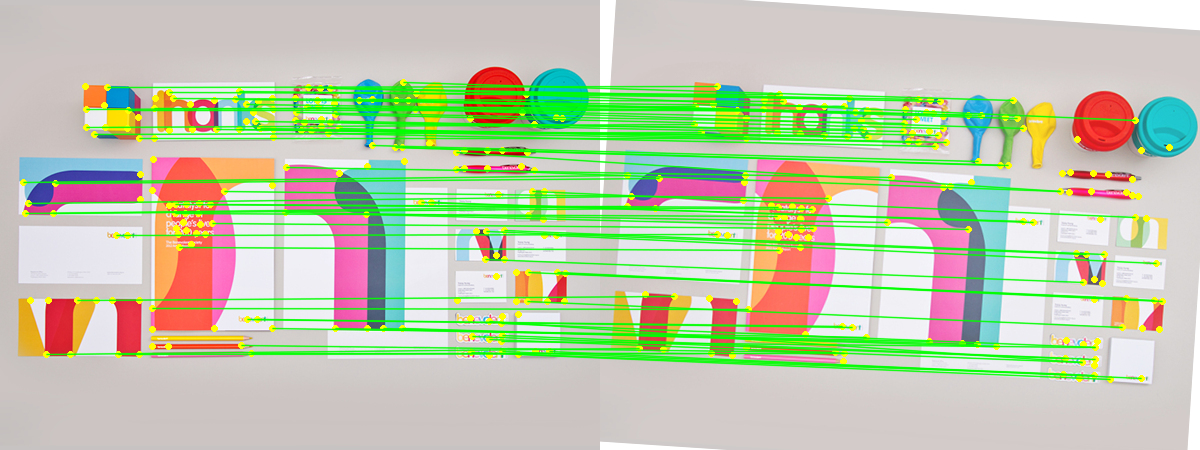
\includegraphics[width=8.9cm,natwidth=1200,natheight=450]{figs/ssd.png}
\label{fig:ssd}
\end{figure} 

\subsection{Normalized Cross-Correlation}
El valor del umbral en NCC se estableció en 0,96
ya que era el que más correspondencias encontraba
sin error. Los valores de correspondencias totales
encontradas se muestran en la tabla \ref{tb:tncc}
y el resultado en la figura \ref{fig:ncc}.

\begin{table}[H]
\centering
\begin{tabular}{*2c}
\toprule
Valor Umbral & Corresp. Detectadas\\
\midrule
0,95 & 101\\
0,96 & 91\\
0,97 & 75\\
0,98 & 56\\
0,99 & 28\\
\bottomrule
\end{tabular}
\caption{Valores de Umbral para NCC.}
\label{tb:tncc}
\end{table} 


\begin{figure}[H]
\caption{Resultado NCC}
\centering
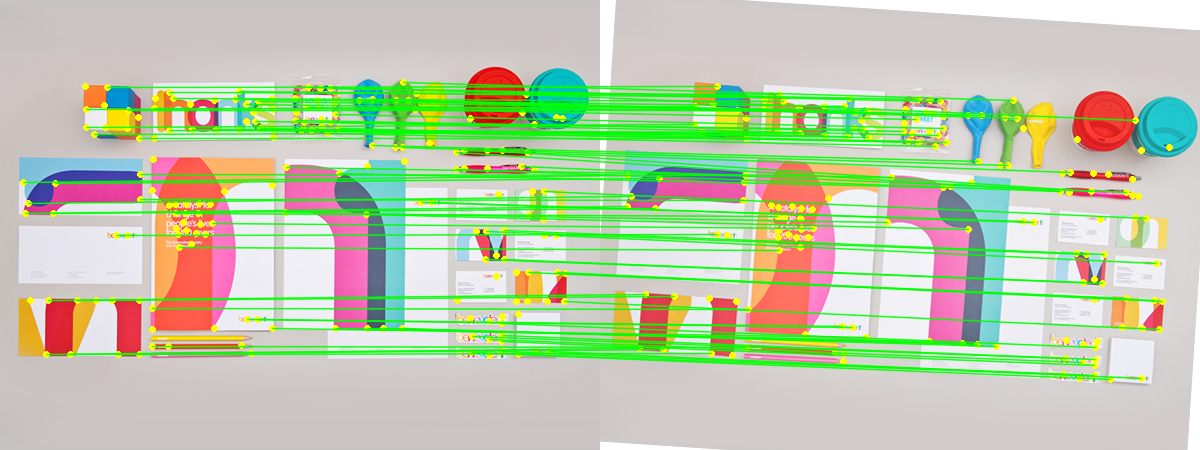
\includegraphics[width=8.9cm,natwidth=1200,natheight=450]{figs/ncc.png}
\label{fig:ncc}
\end{figure} 

\subsection{Comparación}
Usando el método NCC obtuvieron mejores resultados ya que este método es menos sensible a los cambios en la iluminación de la imágen.

Por ejemplo, para la imágen de prueba 1 se hizo una prueba adicional aumentando el
brillo de la imágen. Ante este cambio, el método NCC fue más robusto ya que la 
cantidad de correspondencias detectadas siguió igual, mientras que SSD se redujo 
significativamente.

\begin{table}{H}
\centering
\begin{tabular}{*5c}
\toprule
& \multicolumn{2}{c}{SSD} & \multicolumn{2}{c}{NCC} \\
Iluminación & thold & Matches & Thold & Matches \\ 
\midrule
Similar & 0,30 & 58 & 0,97 & 75 \\
Brillante & 0,30 & 0 & 0,97 & 31 \\
BrillanteMod & 0,80 & 17 & 0,92 & 80 \\
\bottomrule
\end{tabular}
\caption{Parámetros SSD y NCC para variación en luminosidad.}
\label{tb:ssdncc}
\end{table} 

Los de las correspondencias con SSD y NCC sobre la imágen empleando
los parámetros de la última fila de la tabla \ref{tb:ssdncc}
se pueden apreciar en las figuras \ref{fig:ssdlight} y \ref{fig:ncclight}.

\begin{figure}[H]
\caption{Resultado SSD BrillanteMod}
\centering
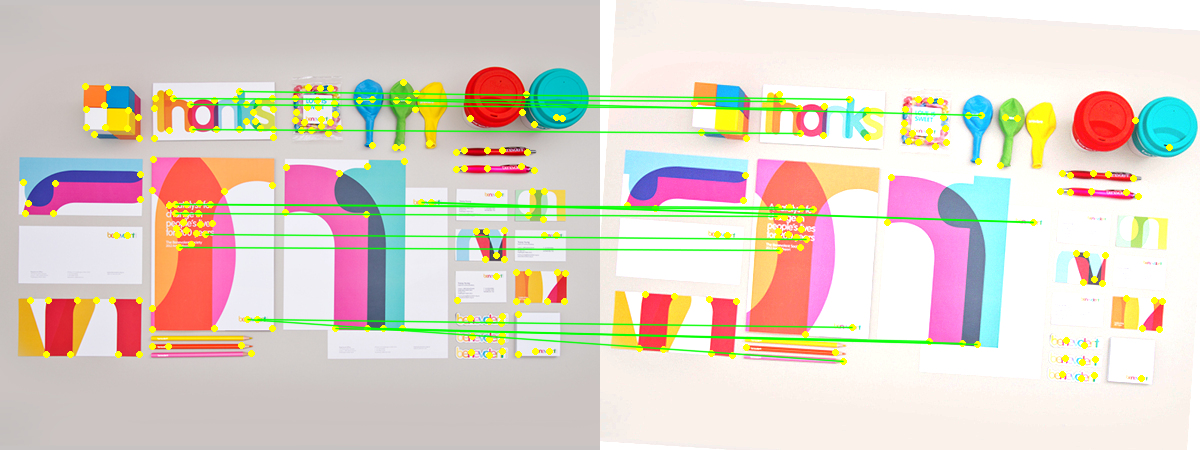
\includegraphics[width=8.9cm,natwidth=1200,natheight=450]{figs/ssdlight.png}
\label{fig:ssdlight}
\end{figure} 

\begin{figure}[H]
\caption{Resultado NCC BrillanteMod}
\centering
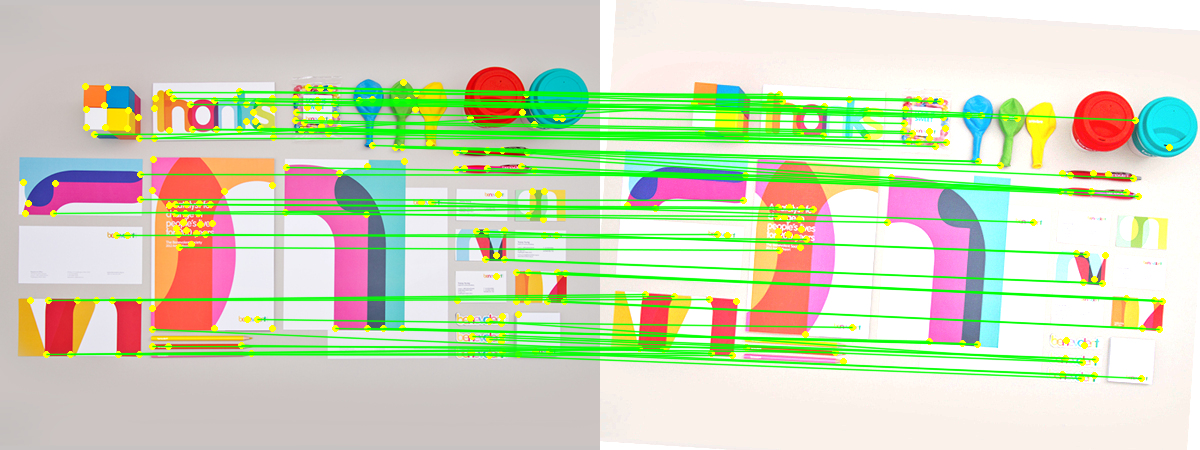
\includegraphics[width=8.9cm,natwidth=1200,natheight=450]{figs/ncclight.png}
\label{fig:ncclight}
\end{figure} 
\section{Otras Pruebas}
A continuación se presentan los resultados obtenidos por el algoritmo
para otros pares de imágenes

\begin{itemize}
\item Prueba 2: Imágen con distorción proyectiva.
\end{itemize} 

\begin{table}[H]
\centering
\begin{tabular}{*2c}
\toprule
Parámetro & Valor \\ 
\midrule
Stdev & 0.60 \\
Harris k & 0.04 \\
Harris WSize & 5 \\
NMS Thold & 0.25 \\
SSD Thold & 1.20 \\
NCC Thold & 0.92 \\
Correspondences WSize & 11 \\
Correspondences knownDisplace & 180 \\
\hline
Harris Corners L & 5925 \\
Harris Corners R & 8788 \\
NMS Corners L & 205 \\
NMS Corners R & 246 \\
SSD Matches & 89 \\
NCC Matches & 79 \\
\bottomrule
\end{tabular}
\caption{Parámetros y Resultados Prueba 2}
\label{tb:test2}
\end{table}

\begin{figure}[H]
\caption{Resultado NCC Prueba 2}
\centering
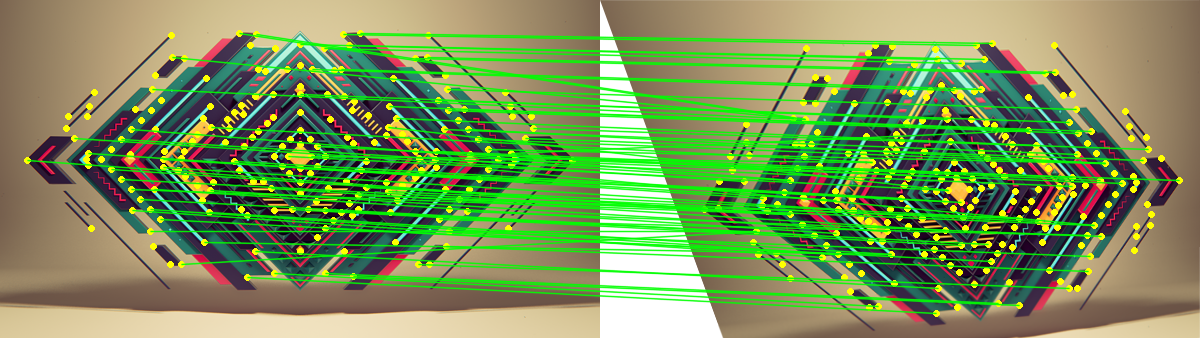
\includegraphics[width=8.9cm,natwidth=1200,natheight=450]{figs/img2ncc.png}
\label{fig:test2ncc}
\end{figure}

\begin{figure}[H]
\caption{Resultado SSD Prueba 2}
\centering
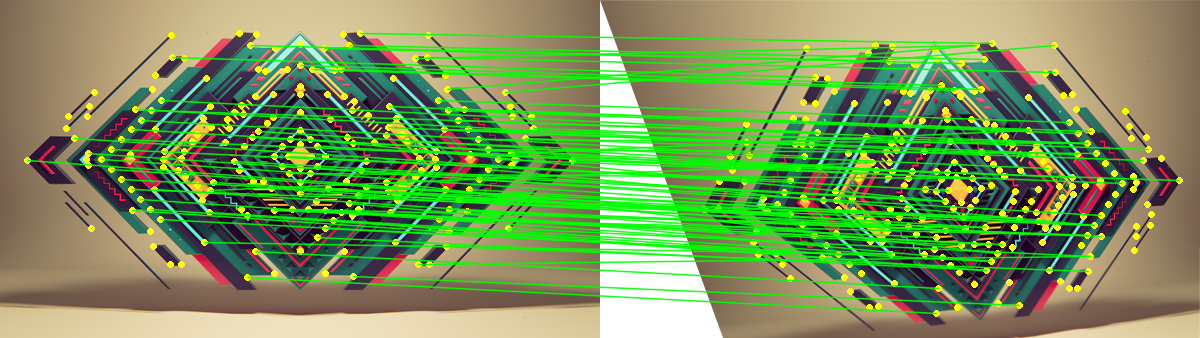
\includegraphics[width=8.9cm,natwidth=1200,natheight=450]{figs/img2ssd.png}
\label{fig:test2ssd}
\end{figure}

\begin{table}[H]
\centering
\begin{tabular}{*2c}
\toprule
Parámetro & Valor \\ 
\midrule
Stdev & 0.60 \\
Harris k & 0.09 \\
Harris WSize & 5 \\
NMS Thold & 0.45 \\
SSD Thold & 0.80 \\
NCC Thold & 0.95 \\
Correspondences WSize & 11 \\
Correspondences knownDisplace & 180 \\
\hline
Harris Corners L & 8218 \\
Harris Corners R & 20294 \\
NMS Corners L & 512 \\
NMS Corners R & 681 \\
SSD Matches & 248 \\
NCC Matches & 255 \\
\bottomrule
\end{tabular}
\caption{Parámetros y Resultados Prueba 3}
\label{tb:test3}
\end{table}

\begin{figure}[H]
\caption{Resultado NCC Prueba 3}
\centering
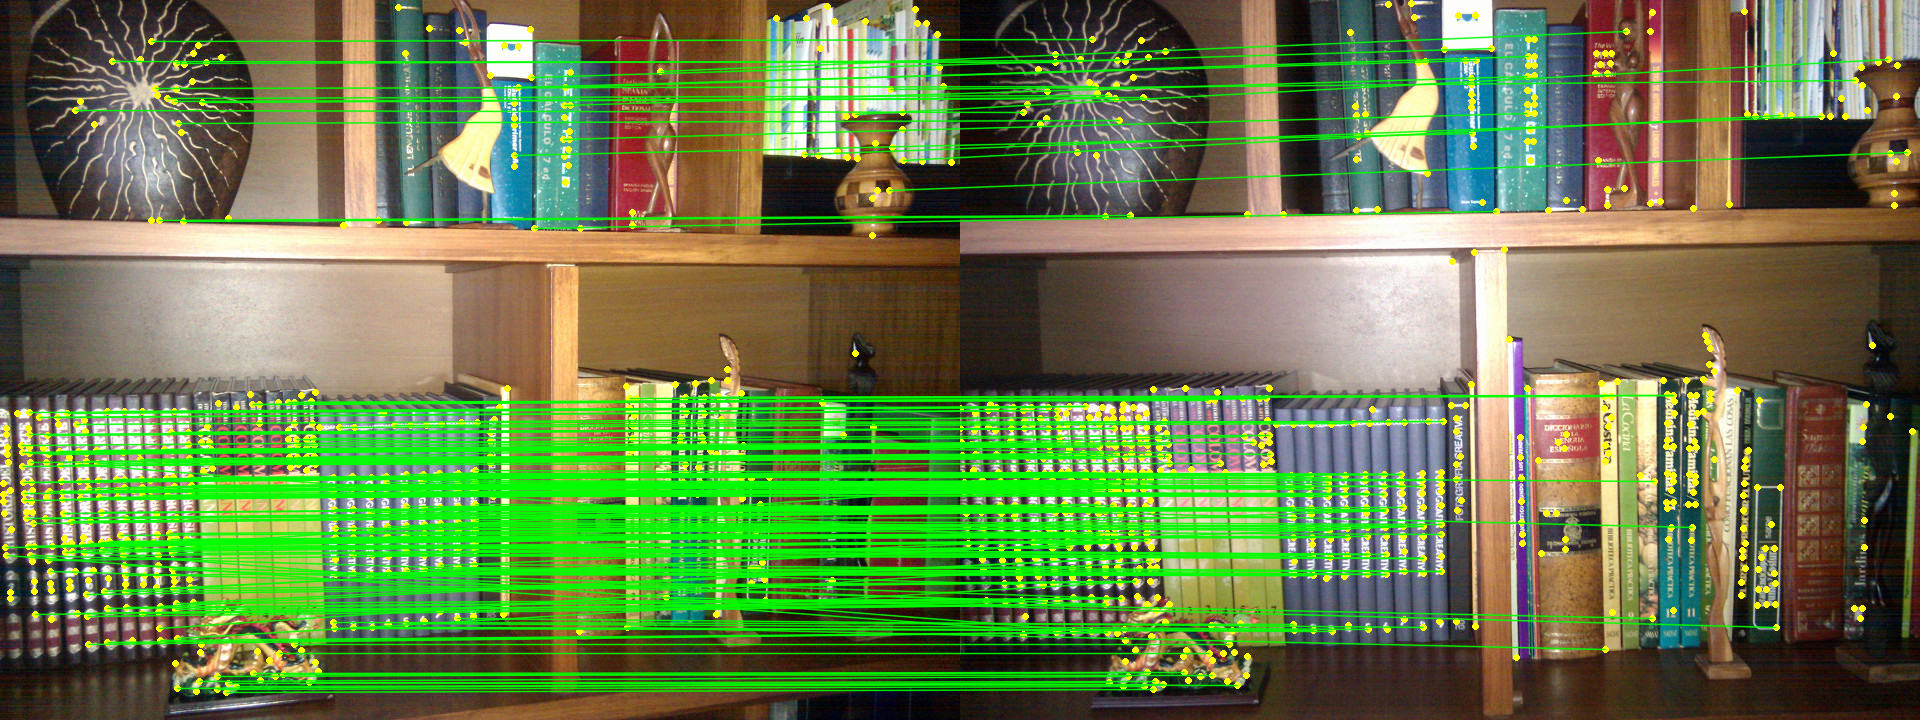
\includegraphics[width=8.9cm,natwidth=1200,natheight=450]{figs/img3ncc.png}
\label{fig:test3ncc}
\end{figure}

\begin{figure}[H]
\caption{Resultado SSD Prueba 3}
\centering
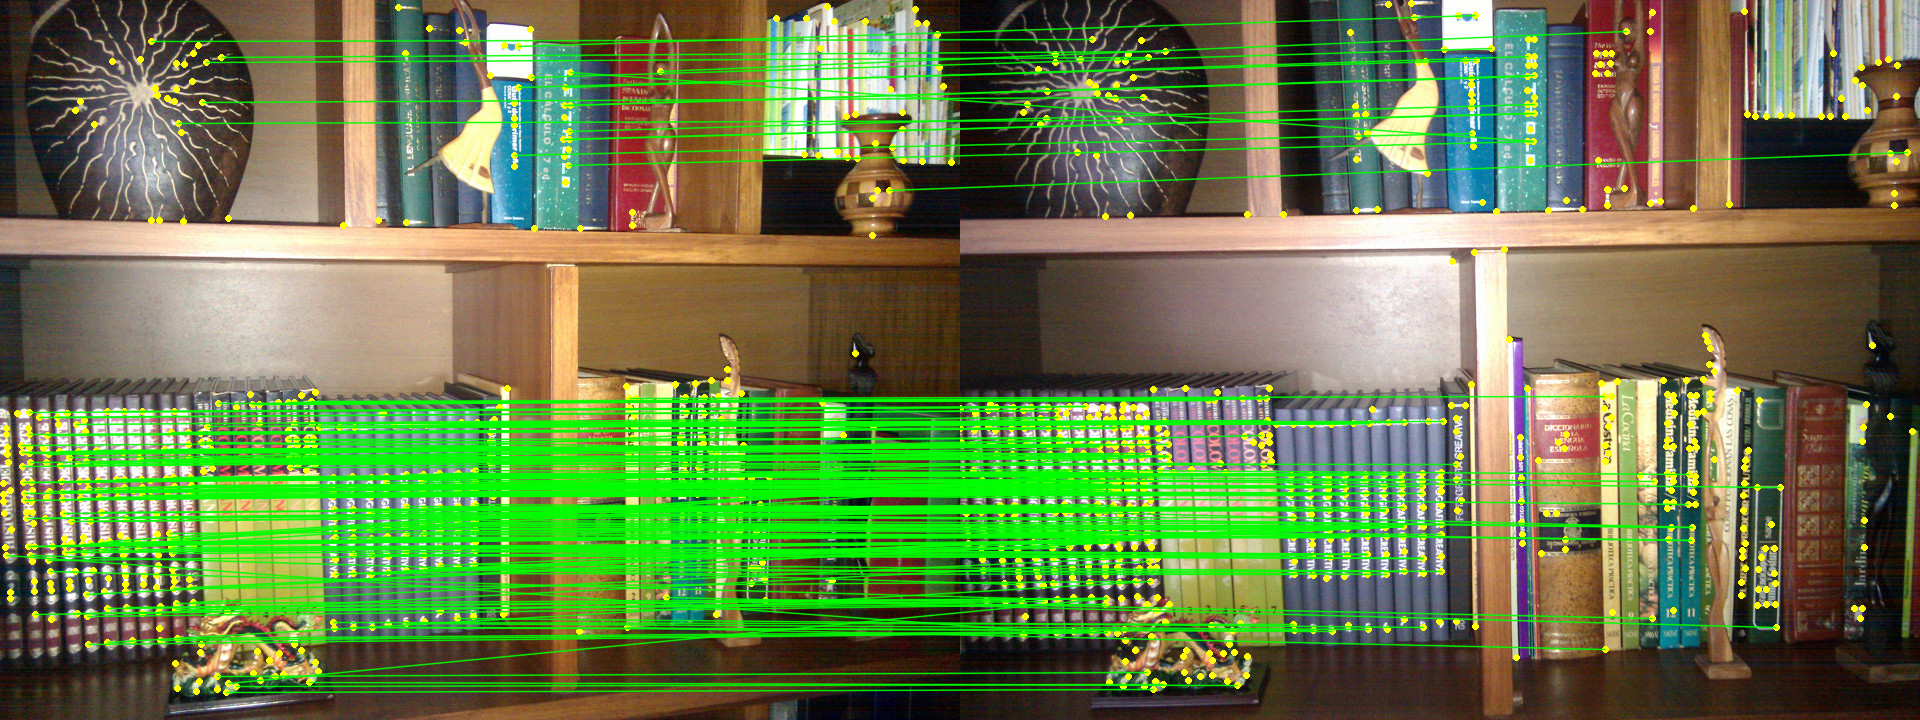
\includegraphics[width=8.9cm,natwidth=1200,natheight=450]{figs/img3ssd.png}
\label{fig:test3ssd}
\end{figure}

\bibliographystyle{plain}
\bibliography{biblio}

\end{document}
